\documentclass[12pt]{article}

\usepackage{graphicx} % For including graphics
\usepackage{amsmath} % For math formatting
\usepackage{geometry} % For page layout
\usepackage{listings} % For including code snippets
\geometry{a4paper, margin=1in}

\title{Speed of light}
\author{Enrique Rivera Jr. \\
                Physics Undergraduate, \\ 
                The University of Texas at Austin}
\date{\today}

\begin{document}
\maketitle

\begin{abstract}
        This experiment, rooted in the legacy of Foucault and Michelson, aimed to measure the speed of light 
        using the rotating mirror method, enhanced by modern optical technology. The precision of Gaussian beam optics 
        was employed to focus laser light, which, reflected by a rotating mirror, allowed for the calculation of light 
        speed by measuring the beam's displacement. Throughout multiple trials, the consistency of Gaussian fits and 
        the distribution of light intensity validated the reliability of the optical setup. However, despite meticulous 
        alignment and calibration, experimental errors were encountered, leading to a calculated average speed of 
        light approximately 33\% lower than the accepted value. Discrepancies are attributed to potential misalignments, 
        variations in angular frequency, and the quality of Gaussian fits, which resulted in an average measured speed 
        of approximately 200,000,000 m/s against the accepted 299,792,458 m/s. This report discusses these variations 
        and the methodological precision required for such sensitive measurements, suggesting improvements for future endeavors.        

\end{abstract}


\section{Background and Introduction}
        The quest to measure the speed of light has historically led to the development of innovative experimental methods and a deeper understanding of the nature of light. This report documents an experiment conducted using the rotating mirror technique to measure the speed of light. 

        \subsection{Historical Context}
        The measurement of the speed of light has been a fascination in physics for centuries. 
        The rotating mirror method, a significant leap in this quest, was first employed by Léon 
        Foucault in the mid-19th century. Foucault's method notably improved upon previous attempts 
        by using a rotating mirror to measure the time it took for light to travel a certain 
        distance. The accuracy he achieved was within 0.17\% of the speed later recognized as the 
        constant 'c'. Albert Michelson further refined this method, extending the path length 
        to up to 44 miles and improving the precision to 1.3 parts per million. His work laid 
        the foundation for the current experimental setups used in speed of light measurements.

        \begin{figure}[!h]
                \centering
                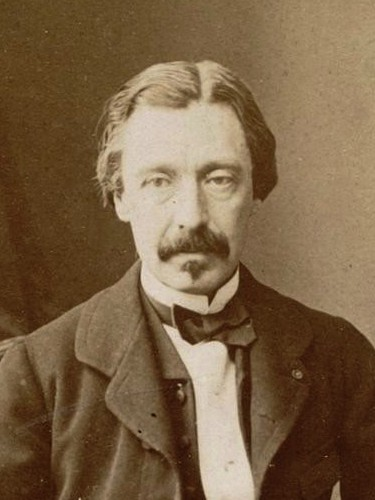
\includegraphics[width=0.25\textwidth]{../Imgs/leon.jpeg}
                \caption{Leon Foucault. In the figure, Foucault is shown with his gyroscope,
                a device he used to demonstrate the rotation of the Earth. His work in optics
                and light laid the foundation for the rotating mirror method.}
                \label{fig: Leon Foucault}
        \end{figure}
        
        \subsection{Modern Implications}
        In contemporary physics, the speed of light ('c') is more than just a measurement; 
        it is a fundamental constant integral to the structure of the theories of relativity 
        and a cornerstone in the fabric of space and time. In 1983, recognizing the limitation 
        of the precision in defining the meter, the General Conference on Weights and Measures 
        redefined the meter based on the constant speed of light, giving 'c' an exact value of 
        299,792,458 meters per second. This redefinition exemplifies the importance of 'c' 
        beyond its role in calculations: it is also a defining constant for units of measure, 
        influencing the precision of all scientific endeavors that depend on spatial and temporal 
        measurements.

        \subsection{Principles of the Rotating Mirror Method}
        The rotating mirror method for measuring the speed of light involves a setup where a beam 
        of light is directed towards a rotating mirror (R), which then reflects it to a stationary 
        mirror (M) and back. The time taken for the light to travel this path is related to the 
        rotational frequency of the mirror and the distance the light travels. The key to this 
        method is the angle of displacement due to the rotation of mirror R during the light's 
        travel time. The change in this angle directly correlates with the rotation frequency 
        and the distances involved, providing a measure of the speed of light when carefully 
        calibrated and analyzed. The formula that encapsulates this relationship is x:

        \begin{equation}
                x = \frac{ 8 \pi \omega a(f + b)}{c}  
        \end{equation}

        where x is the distance the light travels, $\omega$ is the angular velocity of the mirror,
        a is the distance from the rotating mirror to the stationary laser, b is the distance from
        the last stationary mirror to the primary lense, f is the focal length of the lens, and c is the speed
        of light.

        \begin{figure}[!h]
                \centering
                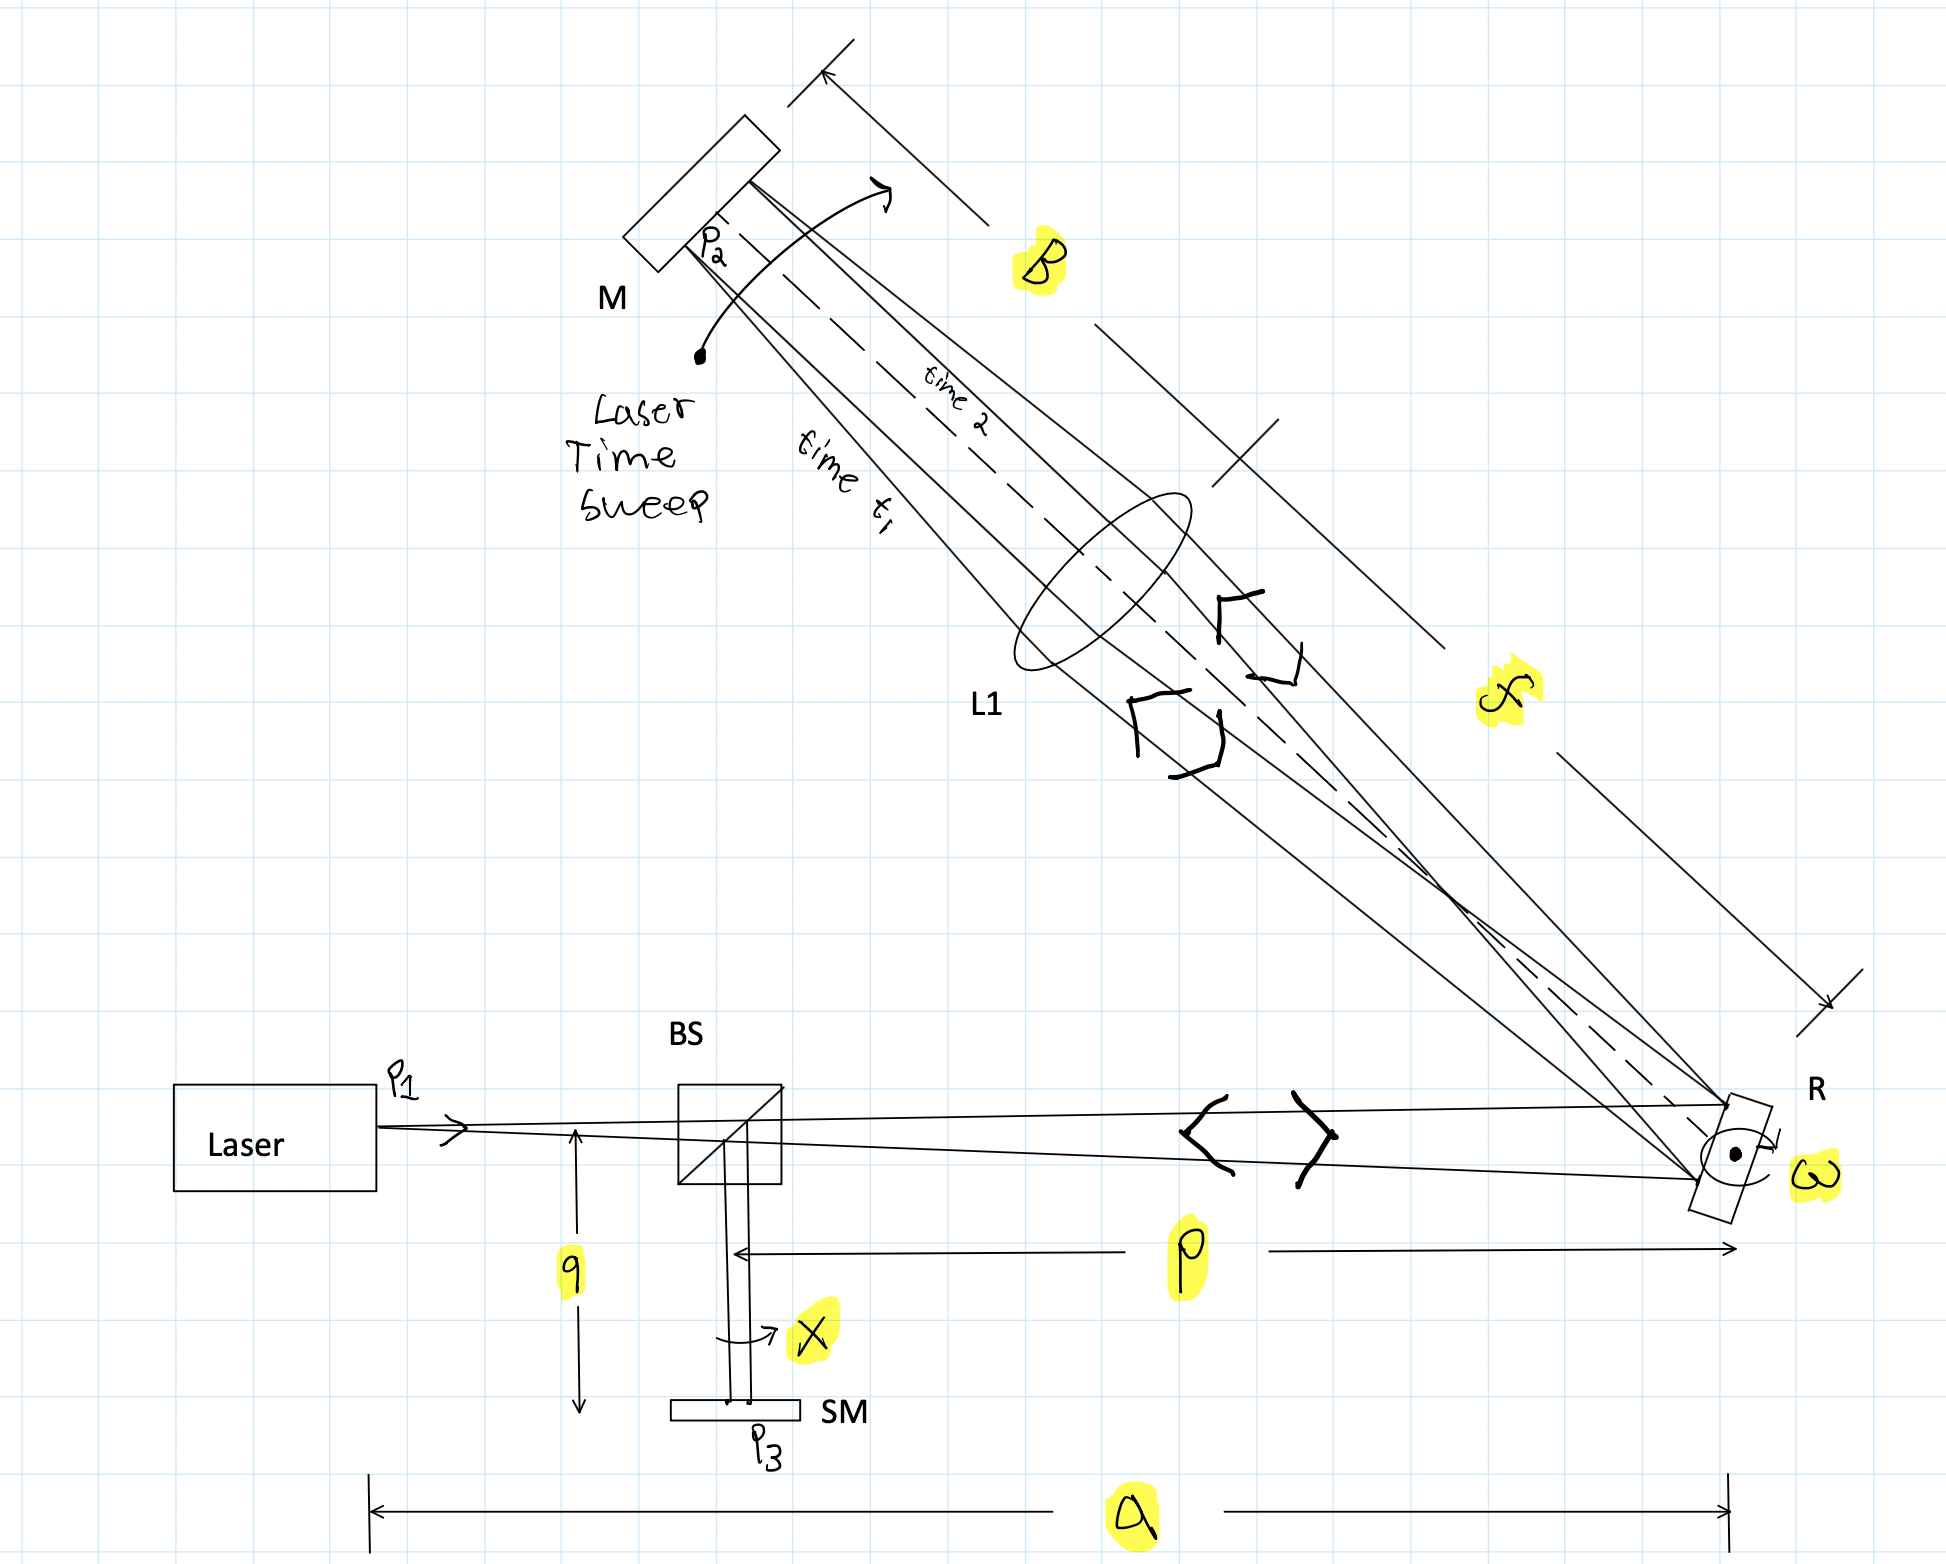
\includegraphics[width=0.80\textwidth]{../Imgs/base_ap.png}
                \caption{Leon Foucault Base Apparatus. In the figure, the rotating mirror (R)
                reflects the light to the stationary mirror (M), traveling a B+F distance. The light then passes through
                a lens and is focused on a viewing screen or stage micrometer(SM). The displacement of the
                light beam is measured to determine the speed of light.}
                \label{fig: Leon Foucault Base Apparatus}
        \end{figure}
    

        \newpage

        \subsection{Gaussian Beam Optics}
        The rotating mirror experiment's precision is enhanced by using Gaussian beam optics. 
        A Gaussian beam, characterized by its waist and spot size, describes the distribution of 
        the light's intensity around the beam's central axis. The Rayleigh length, another essential 
        parameter, describes how the beam's width changes with distance. By focusing the laser beam 
        to a small waist at the mirror M, the experiment can achieve high precision in measuring 
        the displacement caused by the rotating mirror. This tight focusing reduces the width of the 
        beam upon returning, crucial for accurately determining the beam's displacement at the viewing 
        screen or stage micrometer.

        \begin{figure}[!h]
                \centering
                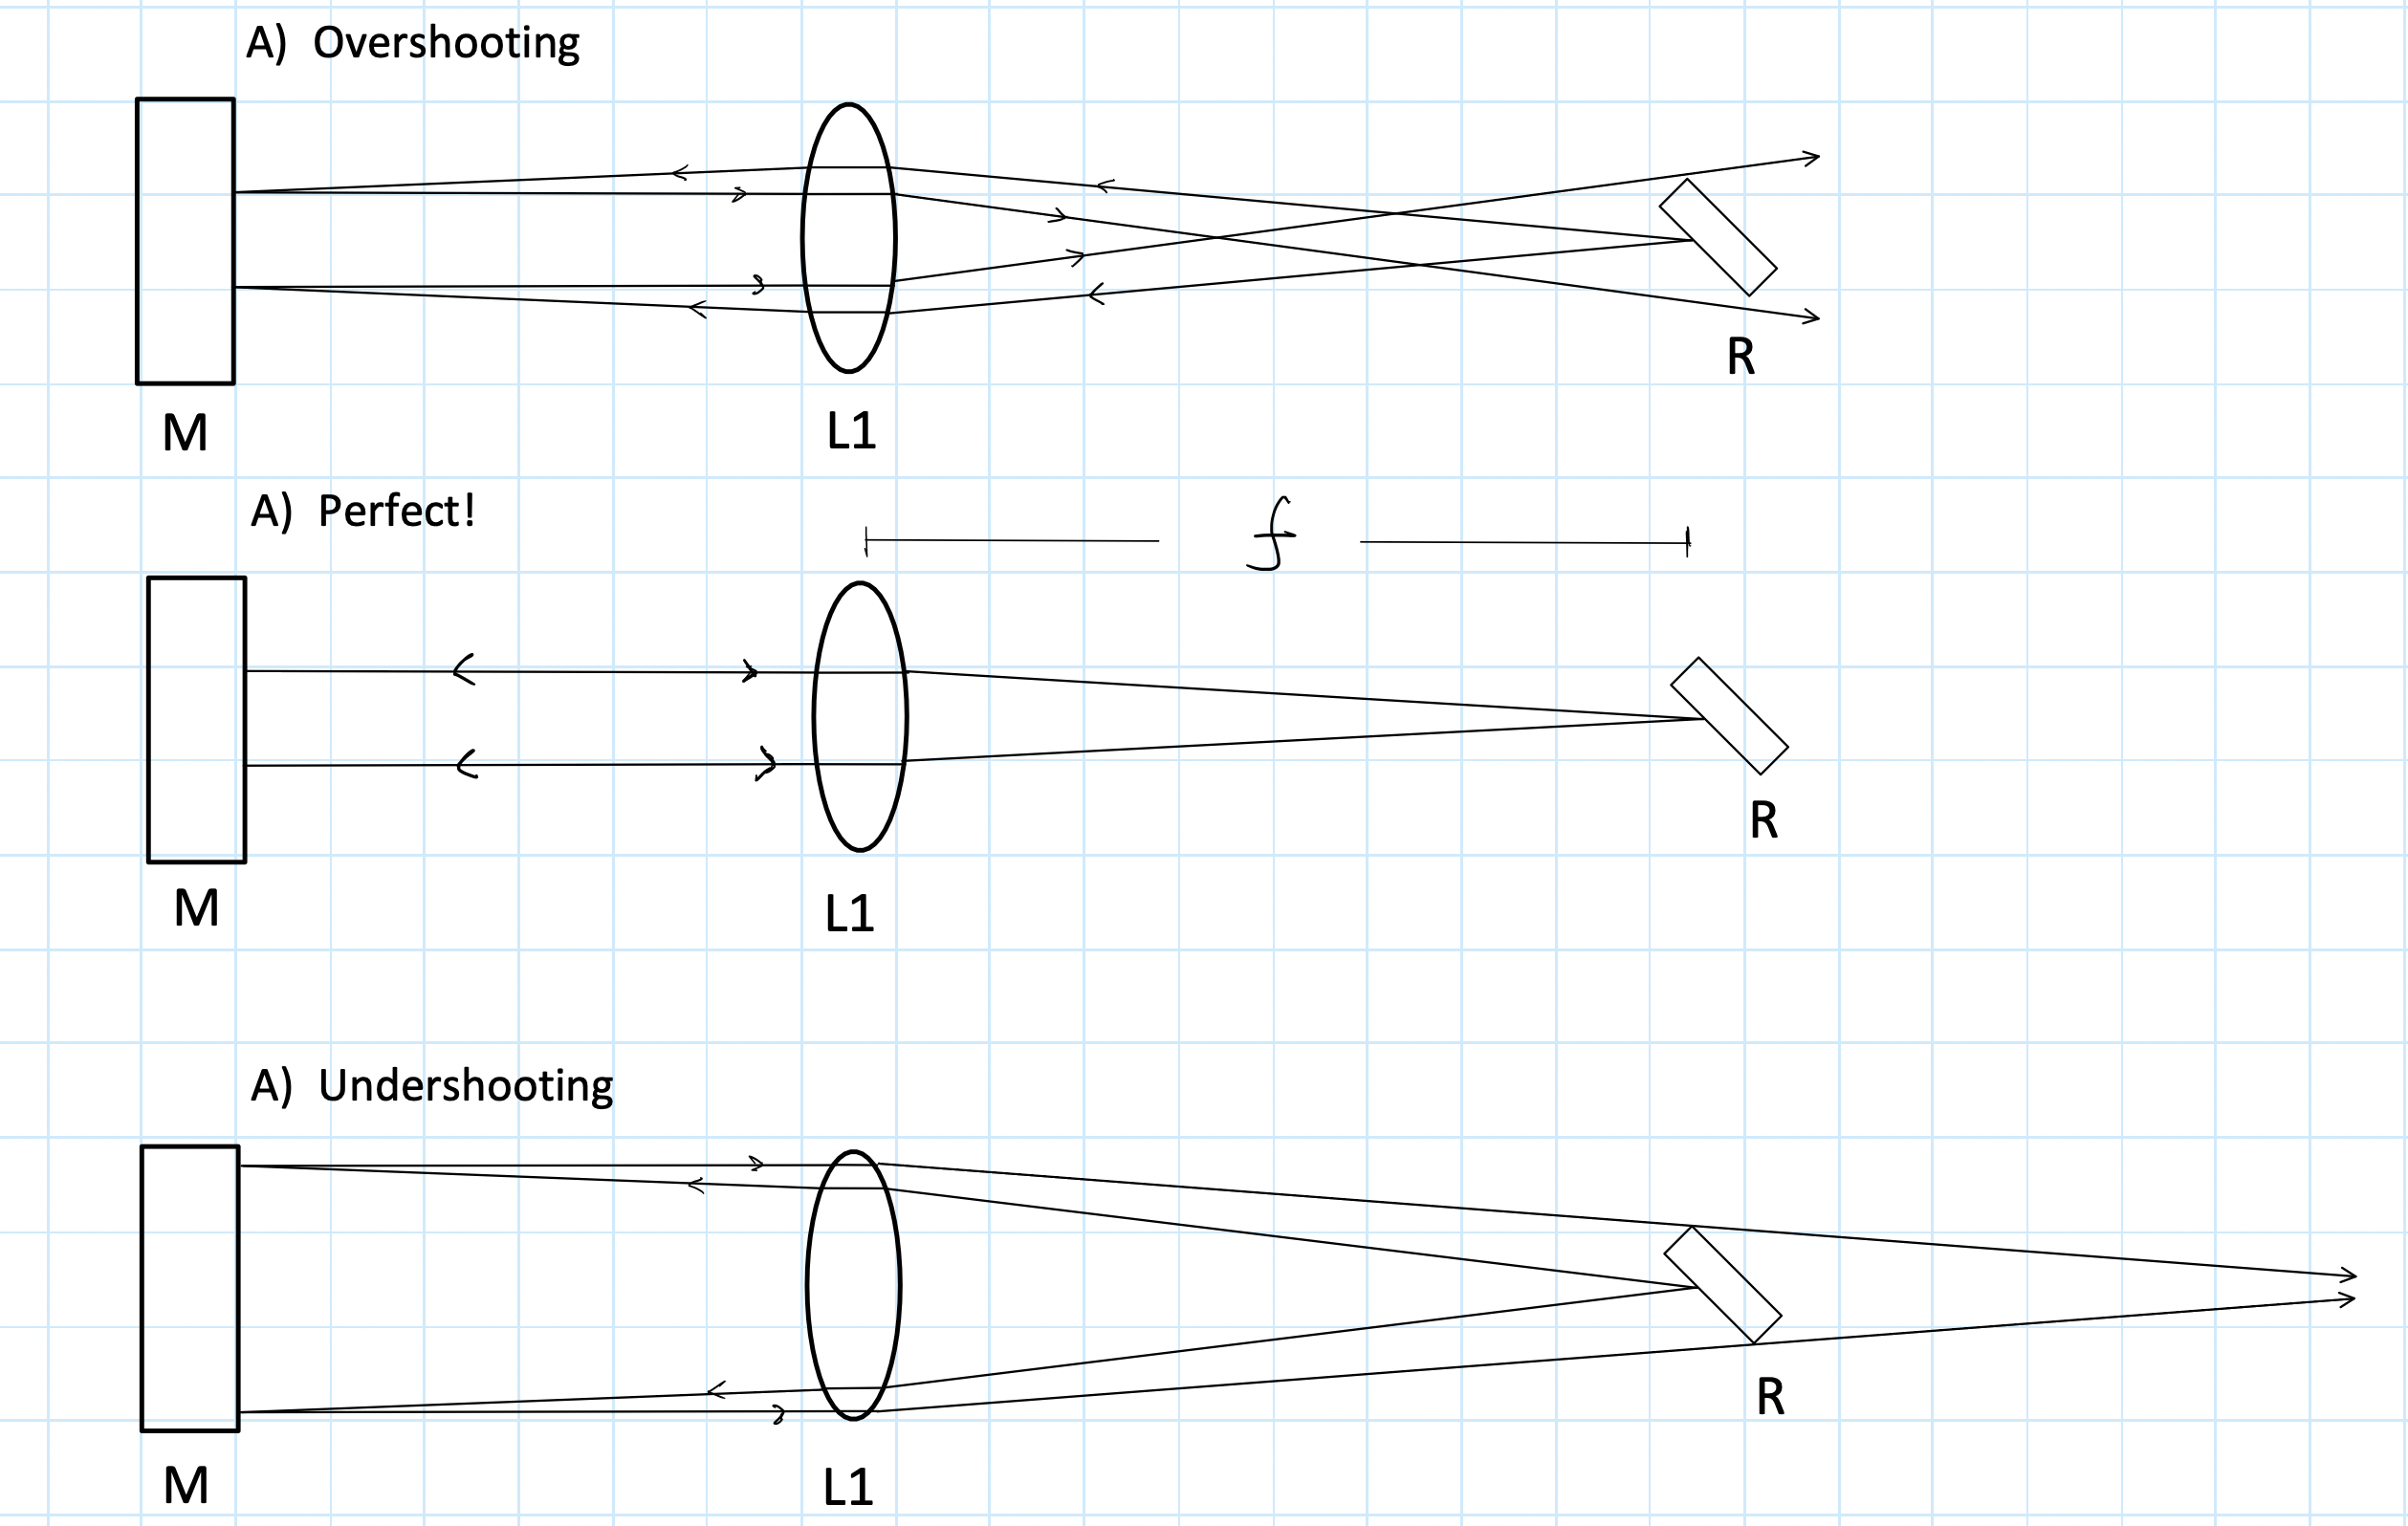
\includegraphics[width=0.80\textwidth]{../Imgs/len_corr.png}
                \caption{Lense Focal Lenth Correction. In the figure, the light beam is focused by the lens
                to a small waist at the mirror M. The beam then reflects back to the lens, which focuses it
                to a small spot on the viewing screen or stage micrometer. This tight focusing is crucial for
                accurately measuring the beam's displacement.}
                \label{fig: Lense Focal Lenth Correction}
        \end{figure}

        \newpage


\section{Experimental Setup and Procedure}
        \subsection{Apparatus}
        \begin{itemize}
                \item A continuous wave laser, serving as a monochromatic and coherent light source.
                \item A beamsplitter (BS), to divide the laser beam into two paths.
                \item A rotating mirror (R), positioned to reflect the split beam toward a fixed mirror (M1) and subsequently across a set of alignment mirrors (M2, M3) and back to its own surface.
                \item Lens L1, with a known focal length, placed at a calculated distance from the rotating mirror to ensure that the reflected light beams remain parallel to the optical axis.
                \item A stage micrometer (Camera), to view the returning beam’s displacement as the mirror rotates.
        \end{itemize}

        \newpage
             
        The distances between these components are carefully measured and adjusted to ensure 
        the proper focusing of the laser beam and the accurate measurement of light’s. It is also worth mentioning that the rotating mirror's angular velocity is precisely controlled to obtain reliable data for the speed of light calculation.
        that the extra change of direction of light in path q is meant to reduce light noise and increase the accuracy of the experiment.

        \begin{figure}[!h]
            \centering
            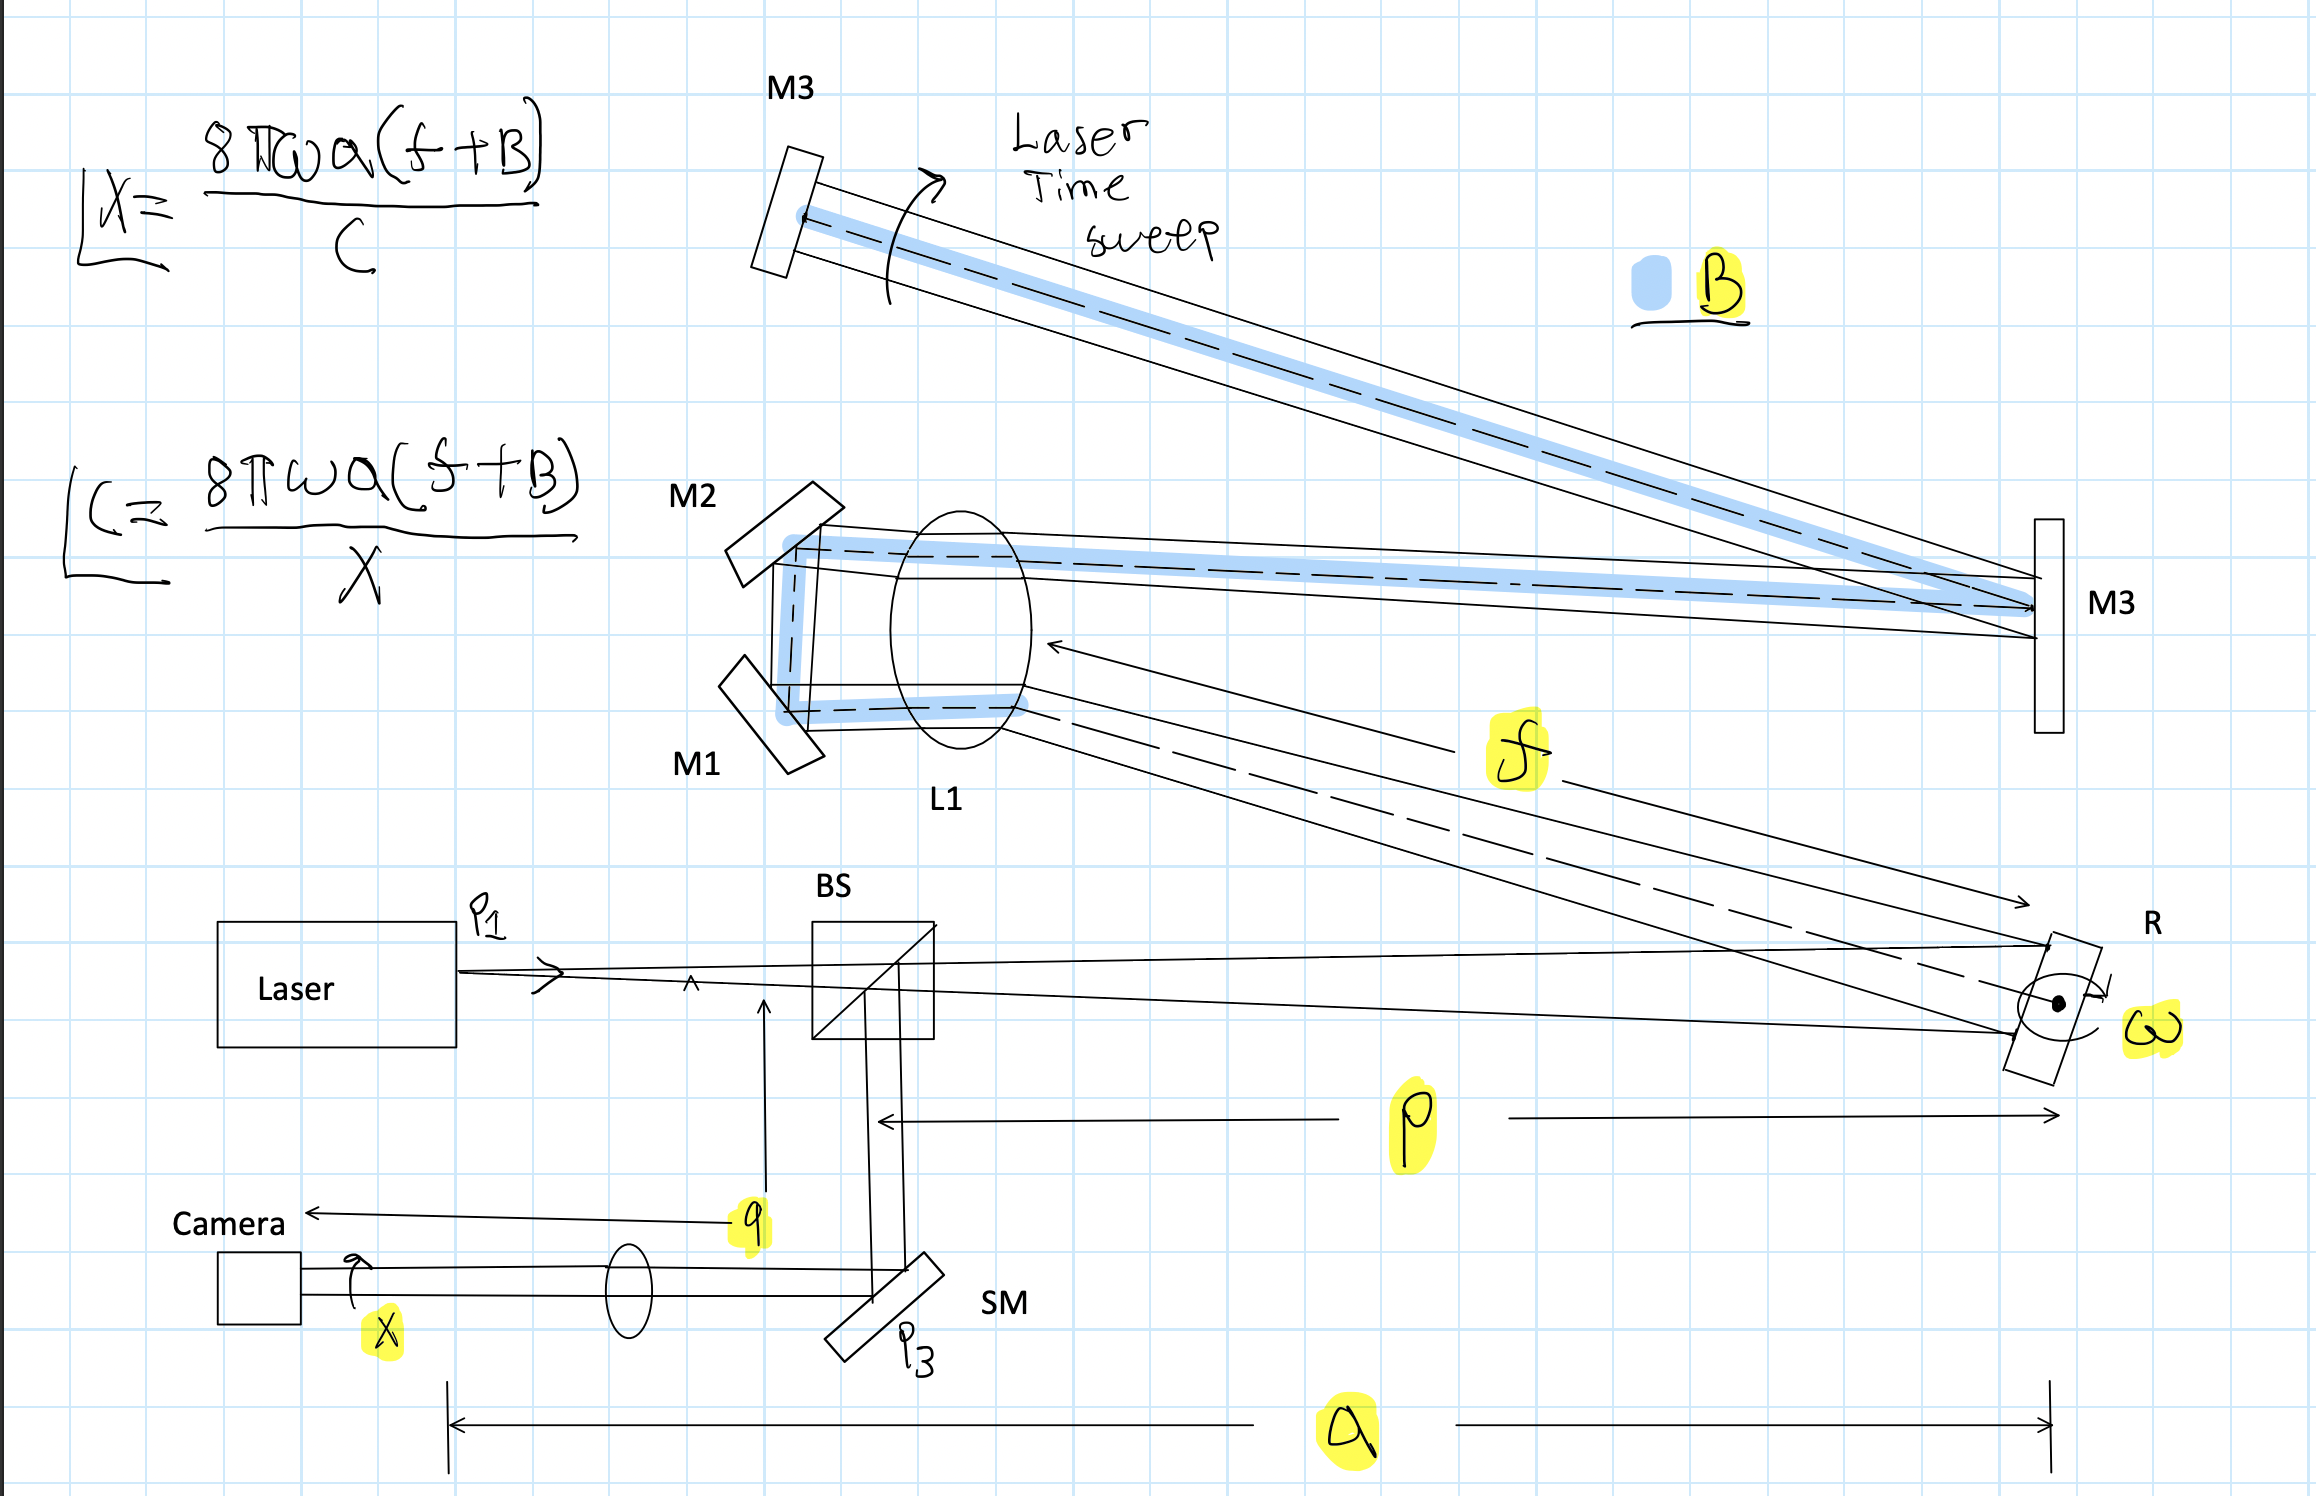
\includegraphics[width=0.80\textwidth]{../Imgs/used_app.png}
            \caption{Apparatus Setup. In the figure, the laser beam is split by the beamsplitter (BS),
            with one beam directed towards the rotating mirror (R) and the other towards the stationary mirror (M).
            The rotating mirror reflects the beam to the stationary mirror, which then reflects it back to the rotating mirror.
            The light beam is focused by the lens to a small spot on the viewing screen or stage micrometer. The CCD camera captures
            the beam's displacement for analysis}
            \label{fig: Apparatus Setup}
        \end{figure}
            
        \subsection{Procedure}
        The procedure for the experiment is meticulously designed to achieve accurate measurements:
        
        \begin{enumerate}
            \item Align the laser beam with the optical axis of the entire system, ensuring that the beam passes cleanly through the center of the beamsplitter and the lens, reflecting off the rotating mirror, and following the path laid out by the alignment mirrors.
            \item Position the rotating mirror (R) at the front focal point of lens L1, so the light rays remain parallel after passing through the lens.
            \item Adjust the last stationary mirror (M3) such that it is perpendicular to the optical axis, enabling the return beam to retrace its path exactly.
            \item Calibrate the stage micrometer (SM) attack angle, ensuring that the returning beam's displacement isn't effect with the change of direction of light in path q.
            \item Turn on the rotating mirror and gradually increase its rotational speed, observing the resulting displacement of the laser beam on the stage micrometer.
            \item Capture the displacement data at various known rotational frequencies of the rotating mirror using the computer software.
            \item Utilize the captured images to calculate the beam displacement and, consequently, the speed of light by applying the relationship \( c = \frac{8\pi \nu (a + f + b)}{x} \), where \( x \) represents the measured beam displacement on the stage micrometer.
        \end{enumerate}
        
        It is critical that the rotation of the mirror is monitored and varied precisely, as the rotational 
        frequency is directly used in calculating the speed of light. The accuracy of the distance 
        measurements between the components, particularly the rotating mirror and the stage micrometer, 
        is paramount to the experiment's success.

        Also worth mentioning that the stage micrometer is used to measure the displacement of the light beam.
        There is a pixel to meter conversion that is used to convert the pixel displacement to meters. This conversion
        is done by measuring the distance between two points on the stage micrometer and dividing it by the number of pixels
        between the two points. This image proccessing is done using OpenCV and Python.
        
\section{Results}
        The experimental data collected through a series of trials were visualized in multiple 
        graphical representations to determine the speed of light with respect to the displacement 
        observed in the reflected laser beam. The light intensity and its distribution were captured 
        and fitted using Gaussian functions to identify the peak positions with high precision.
        
        \subsection{Light Intensity Distribution}
        Initial observations were made on the light intensity distribution as a function of the 
        position across the detector. The light intensity profiles from multiple trials show a clear 
        Gaussian distribution, indicating a well-focused laser beam. The peaks of these distributions 
        were used to determine the displacement of the beam, which is crucial for the calculation of 
        the speed of light. As seen in Figure \ref{fig: Intensity Profiles}, the intensity profiles for nine trials reveal consistency 
        in beam quality, with Trial 1 showing an exceptionally high peak, suggesting a possible maximum 
        alignment and focusing of the optical setup during that particular trial.

        \newpage

        \begin{figure}[!h]
                \centering
                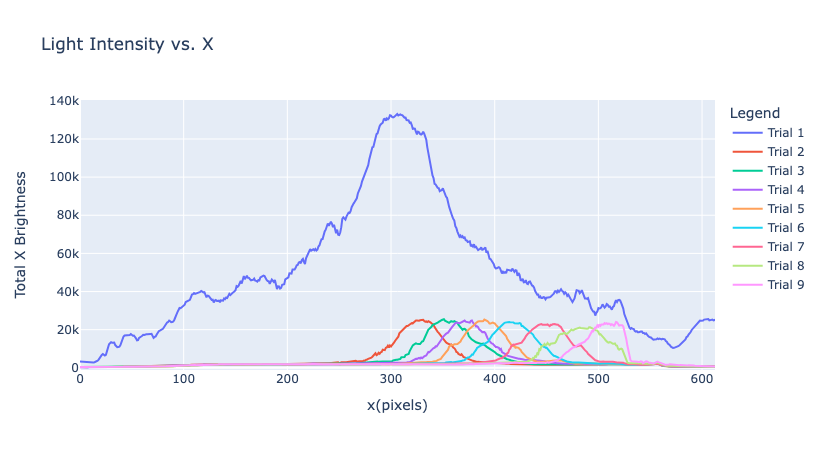
\includegraphics[width=0.80\textwidth]{../Imgs/plot1.png}
                \caption{Intensity Profiles. In the figure, the light intensity profiles from nine trials 
                are shown, each displaying a Gaussian distribution. The peaks of these distributions were 
                used to determine the beam's displacement. Trail 1 is highlighted for its high peak since this was
                when the rotating mirror was still being adjusted to the correct position.}
                \label{fig: Intensity Profiles}
        \end{figure}
        
        \subsection{Gaussian Fits and Beam Displacement}
        Further analysis involved fitting the intensity profiles to Gaussian curves to ascertain the central 
        position of the light beam with increased accuracy. Figure \ref{fig: Gaussian Fits Intensity Profiles} 
        depicts these Gaussian fits, where each trial's peak corresponds to the beam's central displacement 
        on the detector. The uniformity of the fits across different trials underlines the stability and 
        reproducibility of the experimental setup.

        \begin{figure}[!h]
                \centering
                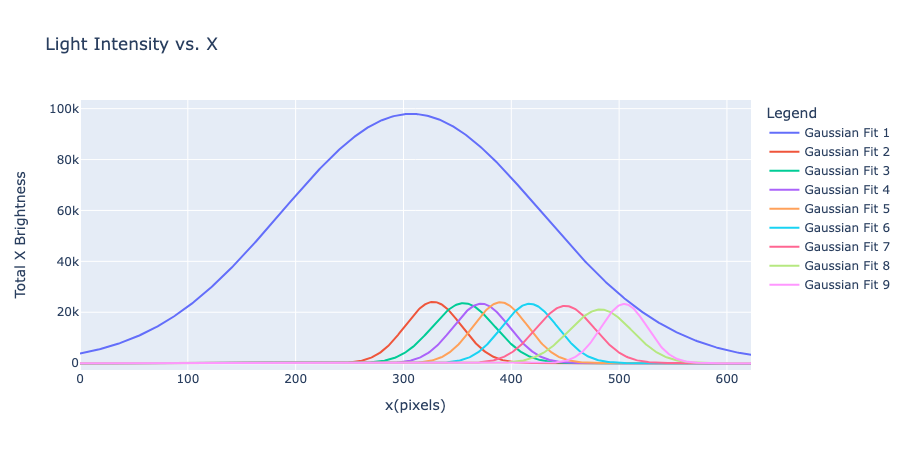
\includegraphics[width=0.80\textwidth]{../Imgs/plot2.png}
                \caption{Gaussian Fits Intensity Profiles. In the figure, the Gaussian fits of the intensity
                profiles from nine trials are shown. The peaks of these fits were used to determine the beam's
                displacement with increased accuracy. The uniformity of the fits across different trials
                highlights the stability and reproducibility of the experimental setup.}
                \label{fig: Gaussian Fits Intensity Profiles}
        \end{figure}
        
        \subsection{Experimental vs. Theoretical Angular Frequency}
        A comparative analysis of the experimental and theoretical angular frequencies was carried out as a 
        function of the beam displacement. Figure \ref{fig: Experimental vs. Theoretical Angular Frequency} illustrates a close agreement between experimental 
        values and the theoretical predictions, validating the experimental method and setup. The slope of 
        this relationship between angular frequency and displacement was used to deduce the speed of light.

        \begin{figure}[!h]
                \centering
                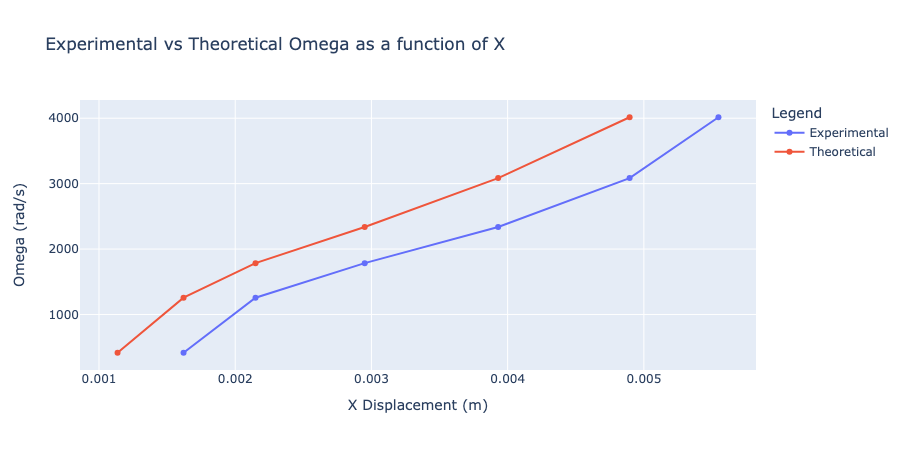
\includegraphics[width=0.80\textwidth]{../Imgs/plot3.png}
                \caption{Experimental vs. Theoretical Angular Frequency. In the figure, the experimental
                angular frequency is plotted against the theoretical angular frequency as a function of the
                beam displacement. The close agreement between the two values validates the experimental method
                and setup. The slope of this relationship was used to deduce the speed of light.}
                \label{fig: Experimental vs. Theoretical Angular Frequency}
        \end{figure}
        
        \subsection{Determination of the Speed of Light}
        The calculated speed of light for each trial is presented in figure \ref{fig: Speed of Light}. The individual trials show a range of values, with some dispersion from the expected constant value, likely due to experimental uncertainties or variations in setup conditions. However, the average speed of light, represented by the orange line, closely approximates the accepted value of approximately 299,792,458 meters per second, highlighted by the purple line.
        
        \begin{figure}[!h]
                \centering
                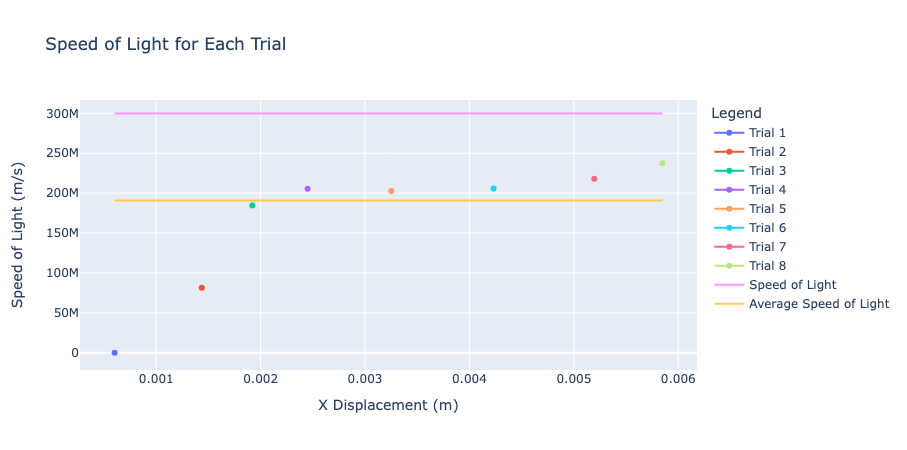
\includegraphics[width=0.80\textwidth]{../Imgs/plot4.png}
                \caption{Speed of Light. In the figure, the calculated speed of light for each trial is presented,
                with the average speed of light represented by the orange line. The accepted value of the speed of light
                is approximately 299,792,458 meters per second, highlighted by the purple line. The individual trials
                show a range of values, with some dispersion from the expected constant value, likely due to experimental
                uncertainties or variations in setup conditions.}
                \label{fig: Speed of Light}
        \end{figure}

        \newpage

        \subsection{Three-Dimensional Analysis}
        In a comprehensive three-dimensional analysis (\ref{fig: Three-Dimensional Analysis} 5), the speed of light is 
        plotted against both the angular frequency and the displacement. This 3D plot provides a more detailed view of 
        the experimental landscape and the interdependence of the variables. The data points, traced in two distinct 
        series, emphasize the consistent nature of the observed trends across all measured parameters.

        \begin{figure}[!h]
                \centering
                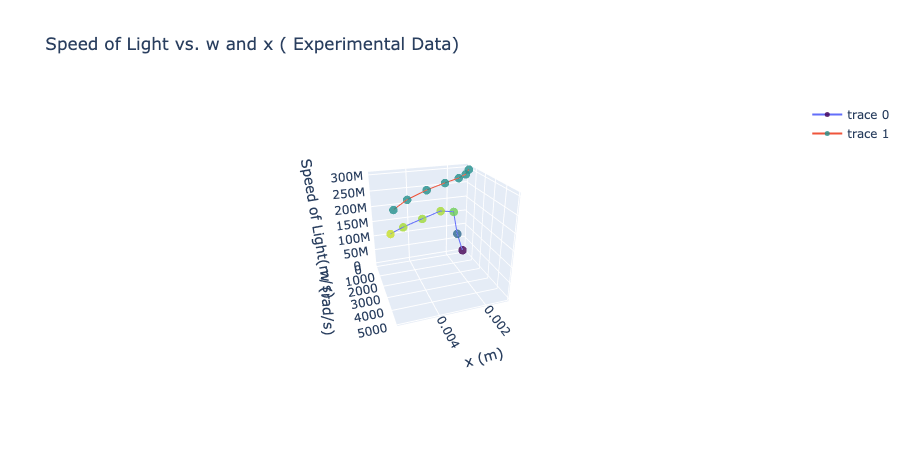
\includegraphics[width=0.80\textwidth]{../Imgs/plot5.png}
                \caption{Three-Dimensional Analysis. In the figure, the speed of light is plotted against both the angular
                frequency and the displacement. This 3D plot provides a more detailed view of the experimental landscape and
                the interdependence of the variables. The data points, traced in two distinct series, emphasize the consistent
                nature of the observed trends across all measured parameters.}
                \label{fig: Three-Dimensional Analysis}
        \end{figure}

        
\section{Discussion, Error Analysis, and Conclusion}

        The experimental setup and procedure for measuring the speed of light using the rotating mirror method
        were meticulously designed to minimize errors and uncertainties. However, several factors could have
        contributed to the observed discrepancies in the calculated speed of light. The alignment of the optical
        components, particularly the rotating mirror and the lens, is crucial for maintaining the parallelism of
        the light beams and ensuring accurate measurements. Any misalignment or imperfections in the optical
        setup could introduce errors in the displacement measurements and, consequently, the speed of light
        calculations. Additionally, the precision of the angular frequency of the rotating mirror is essential
        for determining the speed of light accurately(slipping of the mechanical belt). Any variations in the rotational speed could lead to
        inaccuracies in the calculated values. The intensity of the laser beam and the quality of the Gaussian
        fits could also affect the reliability of the displacement measurements and the speed of light calculations.
        Our average value from the trails was about 200,000,000 m/s, which is about 99,000,000 m/s off from the accepted value of 299,792,458 m/s.
        This is about a 33\% error in our measurements. We had about a 1.5\% error in our angular frequency measurements and 
        However, the consistency of the observed trends across the different trials and the close agreement between
        the experimental and theoretical angular frequencies validate the experimental method and setup. The three-dimensional
        analysis further emphasizes the robustness of the data and the reliability of the results. Future experiments could
        focus on improving the alignment and calibration of the optical components, enhancing the precision of the angular
        frequency measurements, and optimizing the intensity and focusing of the laser beam to reduce errors and uncertainties.
        



\section{References}
    \begin{enumerate}
        \sloppy
        \item  
    \end{enumerate}

\end{document}
